\chapter{SO(3) Regression}
\label{chap:appendix_so3_learning}

\section{Experiments}
\subsection{One-dimensional regression}

\begin{figure*}
	\centering
	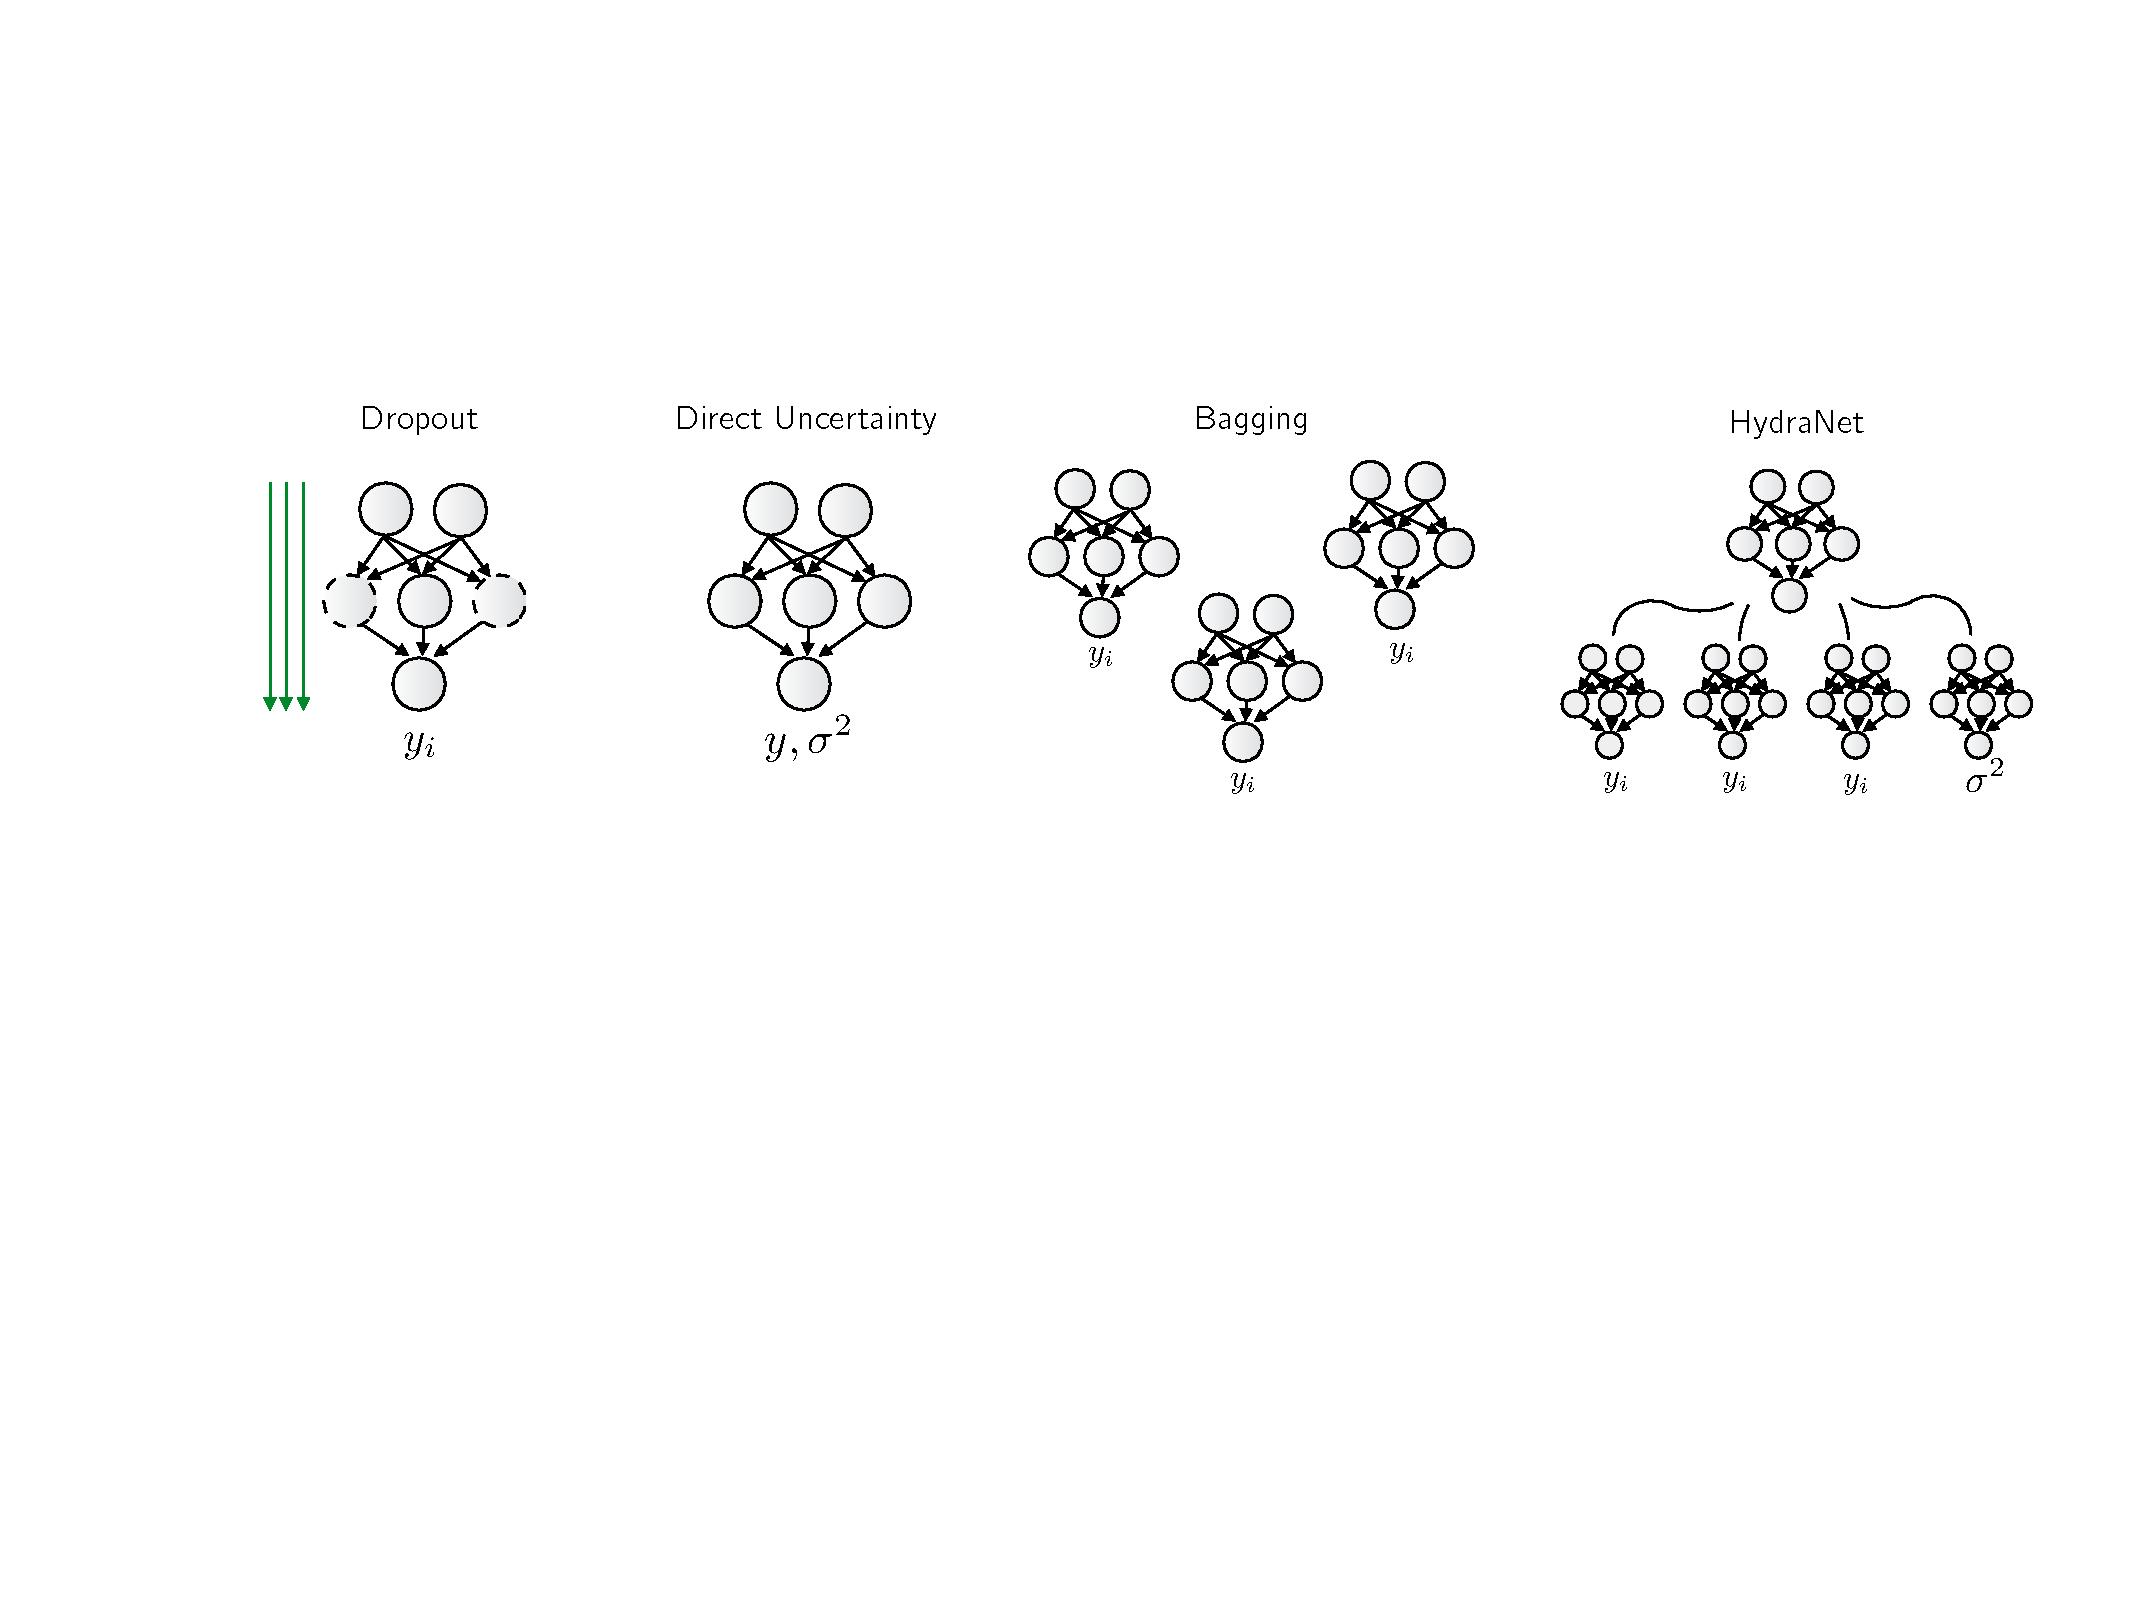
\includegraphics[width=0.98\textwidth]{so3_learning/supplementary/uncertainty_methods.pdf}
	\vspace{-.5em}
	\caption{Different scalable approaches to neural network uncertainty. }
	\label{fig:nn-uncertainty}
\end{figure*}

For each uncertainty extraction, we used a four layer neural network (with 20 units per layer) with a Scaled Exponential Linear Unit (SELU). For the dropout method, we added dropout layers (with a small dropout probability, $p=0.03$, to account for the small network size as recommended by \cite{Gal2016-ny}). We performed 50 forward passes through the network, and computed the mean and variance of the outputs to determine the prediction and uncertainty estimate. For the ensemble bootstrap method, we trained ten separate models on bootstrapped samples of the training data. For HydraNet, we used the first two layers as the body, and branched the final two layers into ten heads.  One additional head was created that directly regressed an uncertainty estimate.  


Every model in this experiment was trained for 3000 epochs using stochastic gradient descent with momentum, using minibatch sizes of 50 (refer to \Cref{tab:1d-hyp} for specific hyper-parameters). We repeated training 100 times, and recorded the test-time negative log likelihood for each method at each repetition.


We present three additional figures here that were not included in the main paper. \Cref{fig:1d_uncertainty} presents four representative samples from the 100 repetitions for each method, and \Cref{fig:1d-mse} presents mean squared errors for each method. The last figure, \Cref{fig:1d-target-noise}, details the effects of adding zero mean Gaussian noise to the regression targets during training. We experimented with this approach to try and promote more diversity amongst the HydraNet heads within training data. We found, however, that although this does improve the negative log likelihoods for HydraNet with only epistemic uncertainty (i.e., the sample variance over the head outputs), its benefits were non-existent for the full HydraNet approach. Namely, since the full HydraNet approach uses an NLL loss, the network tended to account for target noise by enlarging the aleatoric uncertainty rather than overfitting each head to a specific target.

\begin{figure}
	\centering
	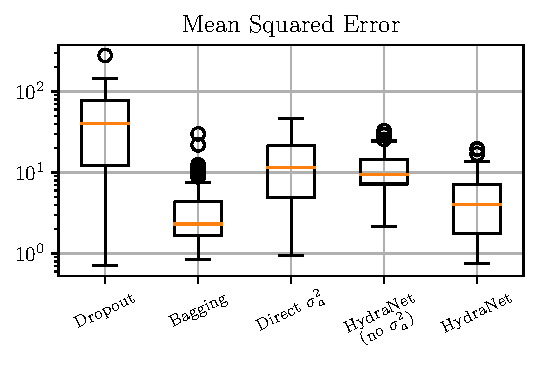
\includegraphics[width=0.48\textwidth]{so3_learning/supplementary/uncertainty-MSE}
	\caption{Mean squared errors for the different probabilistic regression models in 1D.}
	\label{fig:1d-mse}
\end{figure}


\begin{figure}
	\centering
	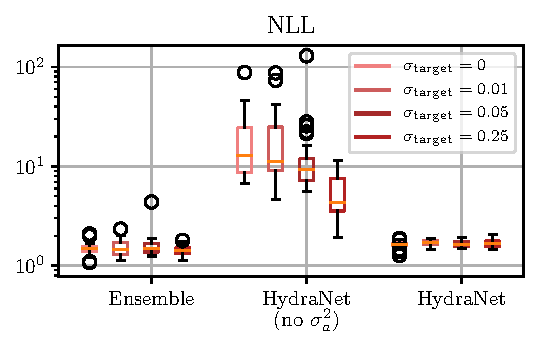
\includegraphics[width=0.48\textwidth]{so3_learning/supplementary/uncertainty-NLL-target_noise}
	\caption{For the 1D experiment, we experimented with adding zero-mean Gaussian additive noise to the regression targets in an attempt to promote diversity amongst the outputs. We found that while this improved the uncertainty estimates gleaned from the HydraNet heads alone (what we call epistemic uncertainty) it made little difference once we included aleatoric uncertainty.}
	\label{fig:1d-target-noise}
\end{figure}


\begin{figure*}[h!]
	%replot images at /so3_learning/1D-uncertainty/replot_experiment_data.py
	%load *.pt to plot a specific run from the 100 run experiment
	\centering
	\begin{subfigure}[]{\textwidth}
		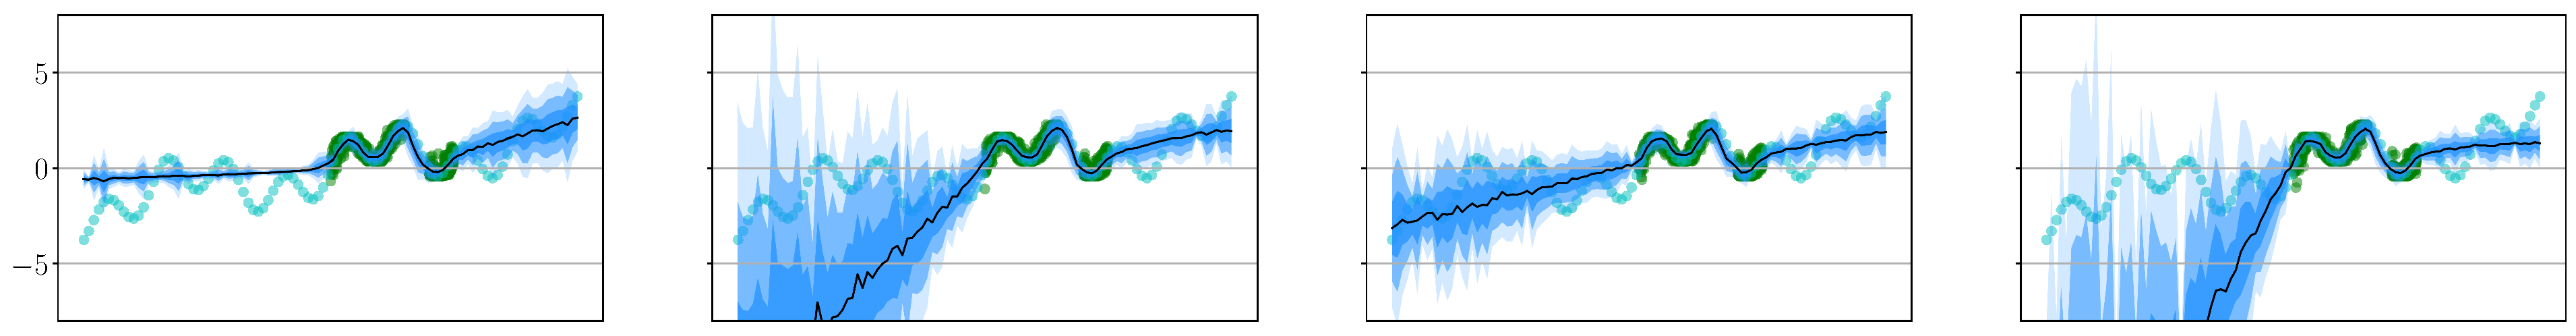
\includegraphics[width=\textwidth]{so3_learning/supplementary/supp_dropout.pdf}
		\caption{Dropout}
		\label{fig:1D_dropout}
	\end{subfigure}
	\hfill
	\begin{subfigure}[]{\textwidth}
		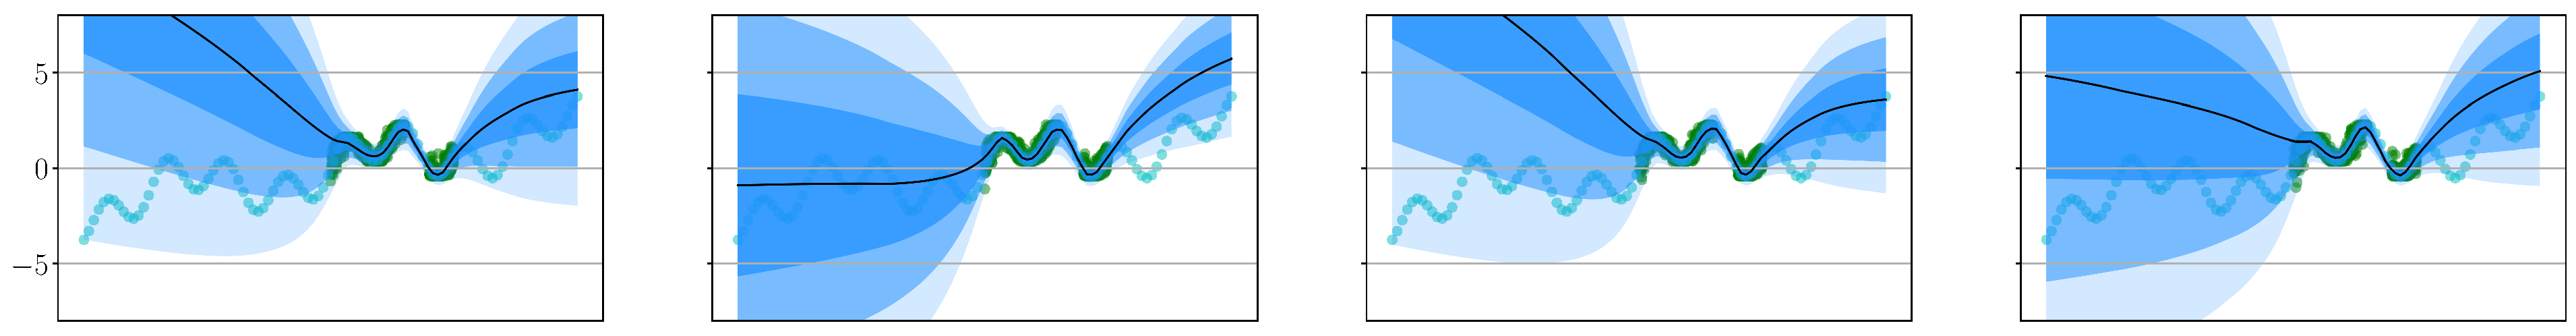
\includegraphics[width=\textwidth]{so3_learning/supplementary/supp_sigma.pdf}
		\caption{Direct Uncertainty}
		\label{fig:1D_direct}
	\end{subfigure}
	\hfill
	\begin{subfigure}[]{\textwidth}
		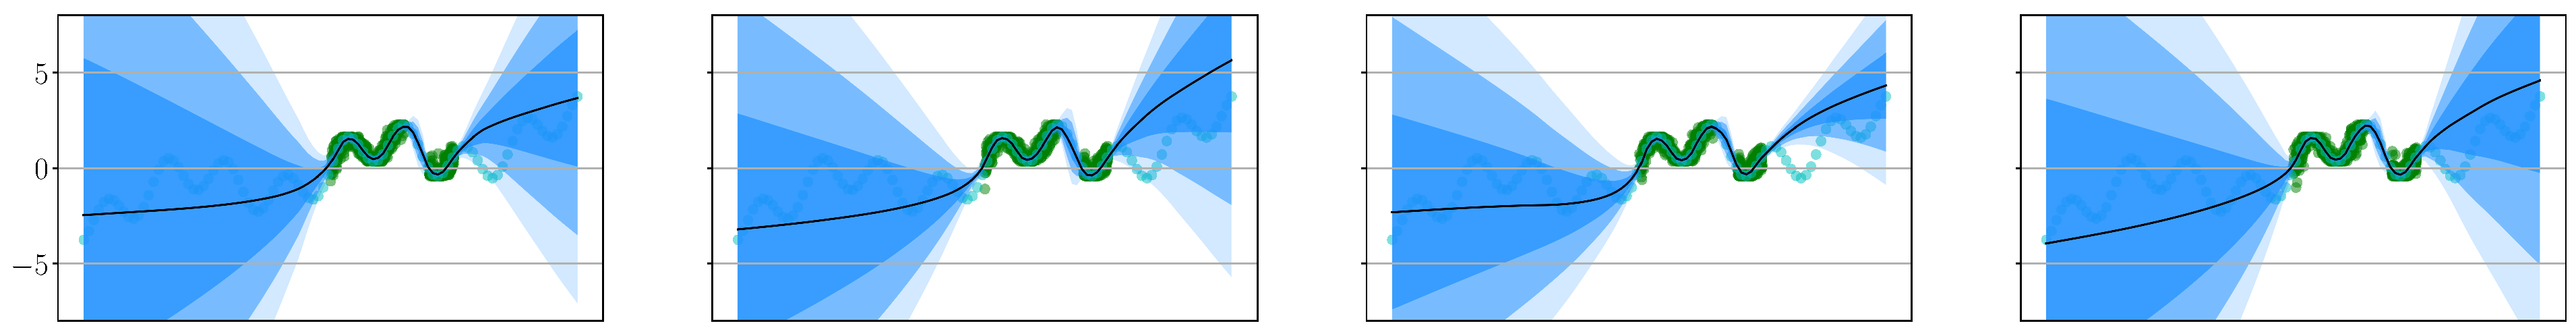
\includegraphics[width=\textwidth]{so3_learning/supplementary/supp_bagging.pdf}
		\caption{Bagging}
		\label{fig:1D_bagging}
	\end{subfigure}
	\hfill	
	\begin{subfigure}[]{\textwidth}
		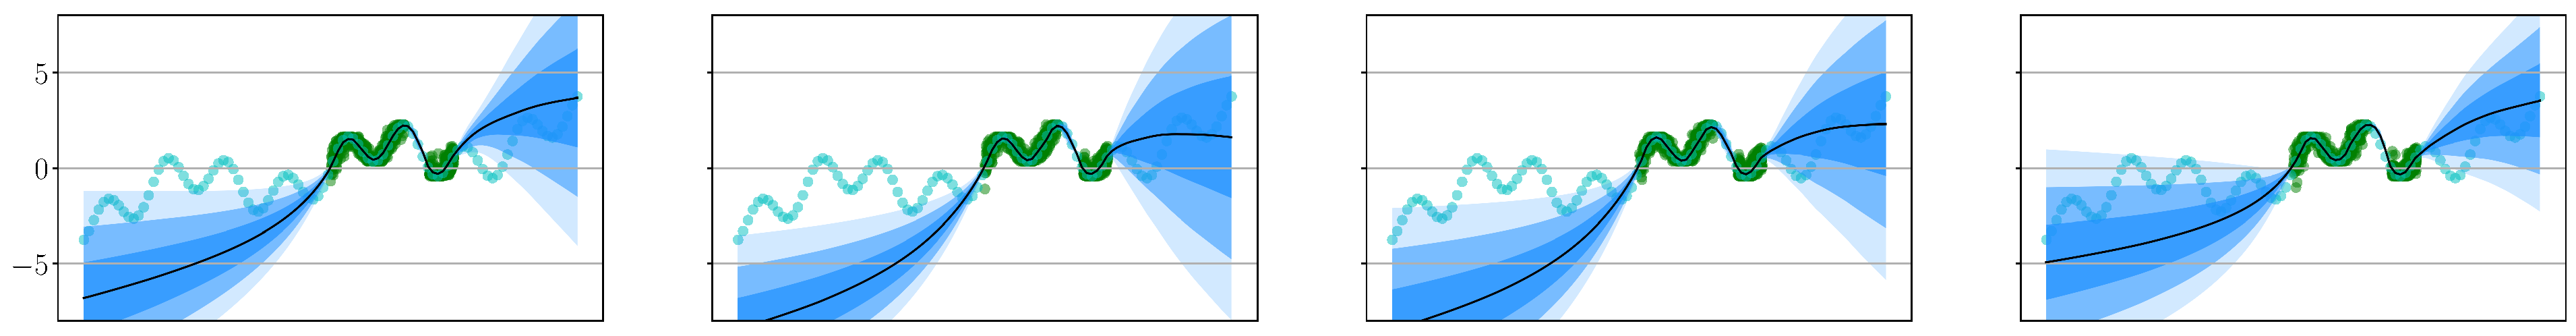
\includegraphics[width=\textwidth]{so3_learning/supplementary/supp_hydranet.pdf}
		\caption{HydraNet (no direct uncertainty)}
		\label{fig:1D_hydranet_undirect}
	\end{subfigure}
	\hfill
	\begin{subfigure}[]{\textwidth}
		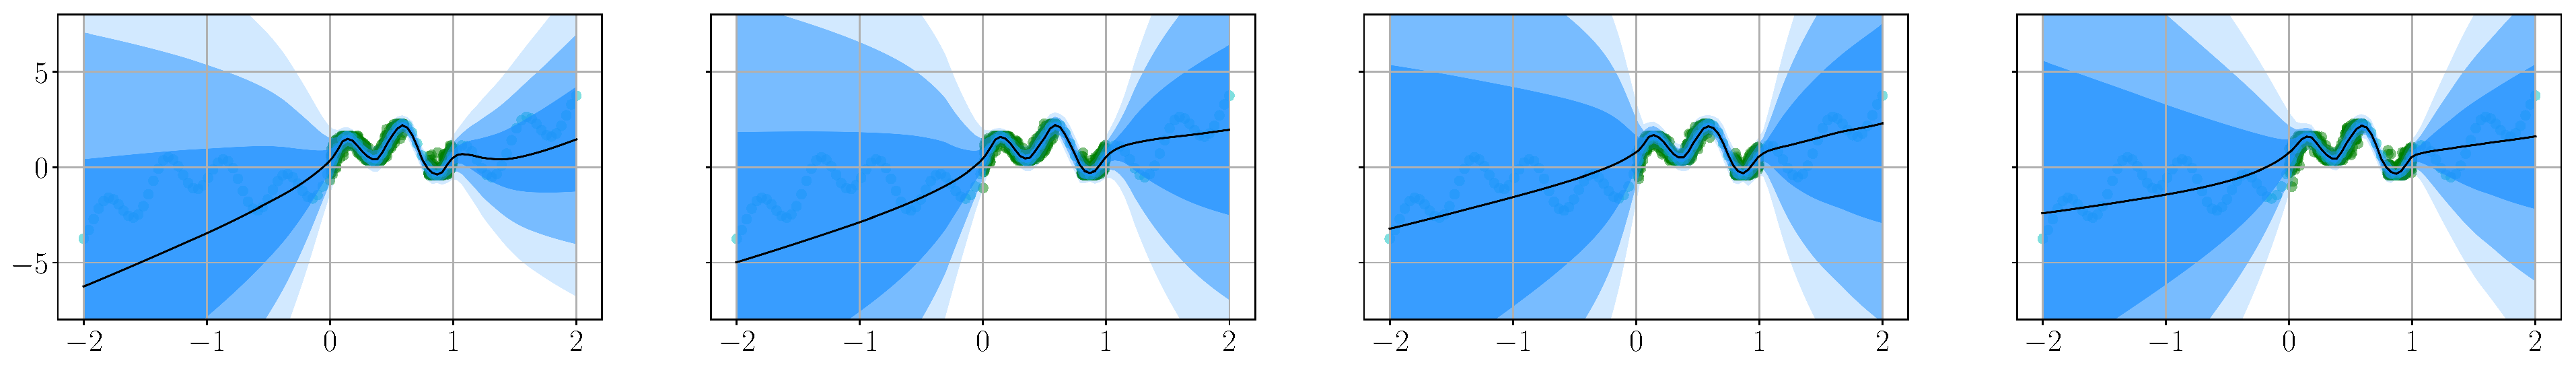
\includegraphics[width=\textwidth]{so3_learning/supplementary/supp_hydranetsigma.pdf}
		\caption{HydraNet}
		\label{fig:1D_hydranet}
	\end{subfigure}
	\hfill		
	\caption{A comparison of different ways to extract uncertainty from deep networks. Each shade of blue represents one standard deviation $\sigma$ produced by the model.}
	\label{fig:1d_uncertainty}
	%\vspace{-0.2cm}
\end{figure*}

\begin{table*}[]
	\centering
	\caption{Hyper-parameters for 1D training.}
	\begin{threeparttable}
	\begin{tabular}{lccc}
		\toprule
		\textbf{Uncertainty Method} & \textbf{Learning Rate} & \textbf{Momentum} & \textbf{Dropout (\%)} \\ \midrule
		Dropout & 0.05 & 0.5 & 3 \\
		Direct Regression & 0.0001 & 0 & 0 \\
		Bagging & 0.01 & 0.9 & 0 \\
		HydraNet (no direct uncertainty) & 0.01 & 0.9 & 0 \\
		HydraNet & 0.01 & 0.1 & 0 \\ \bottomrule
	\end{tabular}
	\label{tab:1d-hyp}
\end{threeparttable}
\end{table*}


\subsection{Hemisphere world}

For this experiment, we created a synthetic world with a 6 $\times$ 6 grid of landmarks, each spaced one meter apart. Our monocular camera resided on a hemisphere (of radius 25 meters) from the centre of the landmark grid. The camera sensor was 500 $\times$ 500 pixels, with a principal point in the middle of the sensor and a focal length of 500 pixels.  We added zero-mean Gaussian noise of unit pixel variance to each landmark projection. 

The network consisted of five residual blocks, each containing a fully connected layer and a ReLU non-linearity. For each camera location, we projected all 36 landmarks onto the image plane, added noise, and then stored 72 image coordinates as training or test input. 

\subsection{7-Scenes}

\Cref{fig:7scenes_regression} presents regression results on all seven scenes from the 7-scenes dataset. Our model consisted of a \texttt{resnet34} body (pre-trained, but not frozen) with 25+1 heads in the same structure as the synthetic experiment. We used the Adam optimizer with a learning rate of $5 \times 10^{-5}$ for all scenes, and trained each model for 15 epochs, selecting the one with the lowest negative log likelihood.

\begin{figure*}[h!]
	\centering
	\begin{subfigure}[]{0.33\textwidth}
		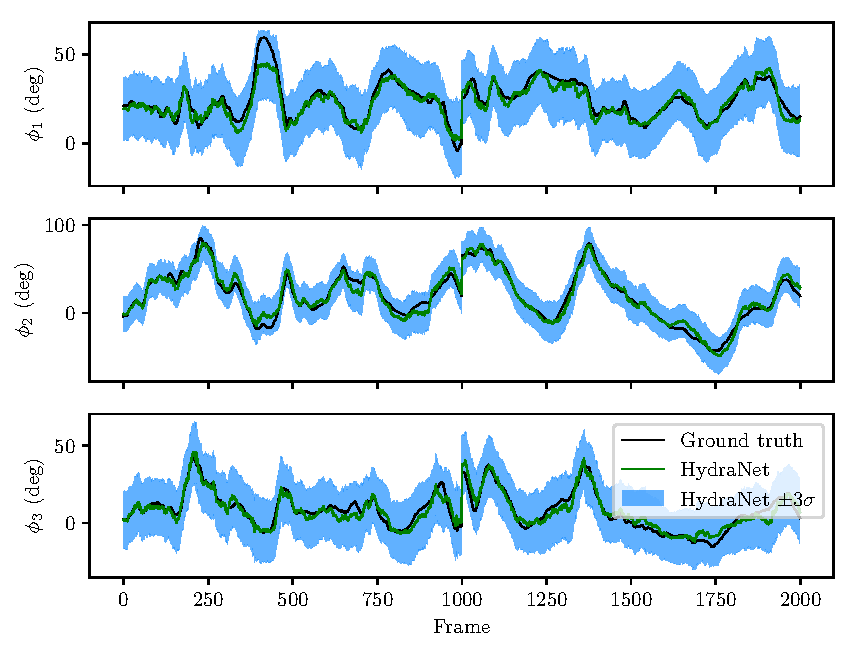
\includegraphics[width=\textwidth]{so3_learning/supplementary/7scenes_abs_best_model_chess_heads_25_epoch_13}
		\caption{Chess}
	\end{subfigure}
	\begin{subfigure}[]{0.33\textwidth} 
		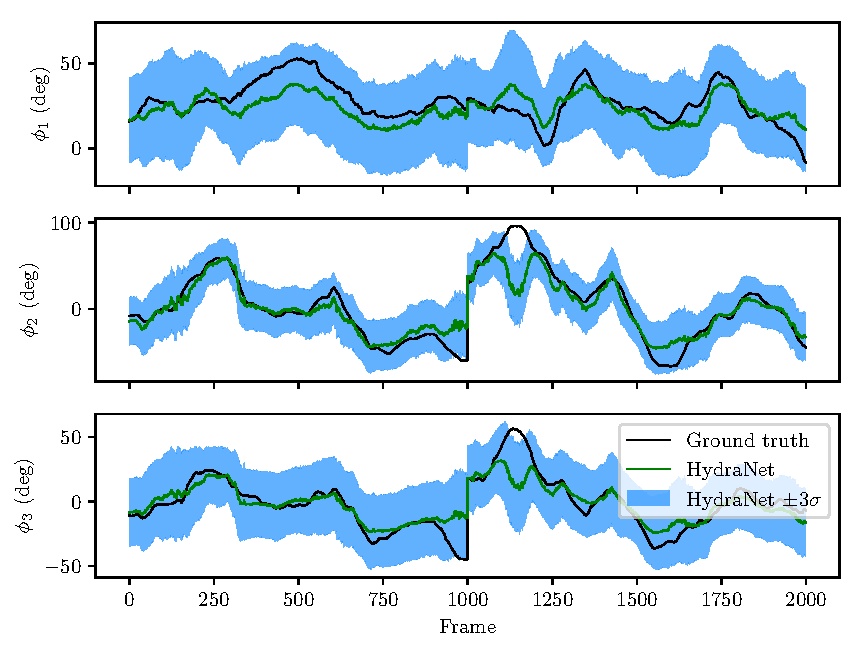
\includegraphics[width=\textwidth]{so3_learning/supplementary/7scenes_abs_best_model_fire_heads_25_epoch_4}
		\caption{Fire}
	\end{subfigure}
	\begin{subfigure}[]{0.33\textwidth} 
		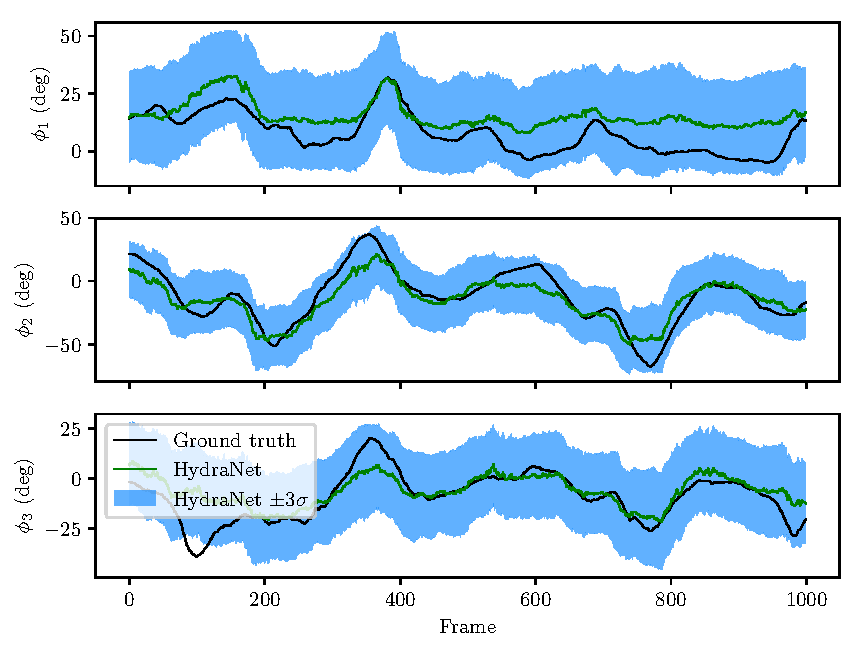
\includegraphics[width=\textwidth]{so3_learning/supplementary/7scenes_abs_best_model_heads_heads_25_epoch_11}
		\caption{Heads}
	\end{subfigure}
	\begin{subfigure}[]{0.33\textwidth} 
		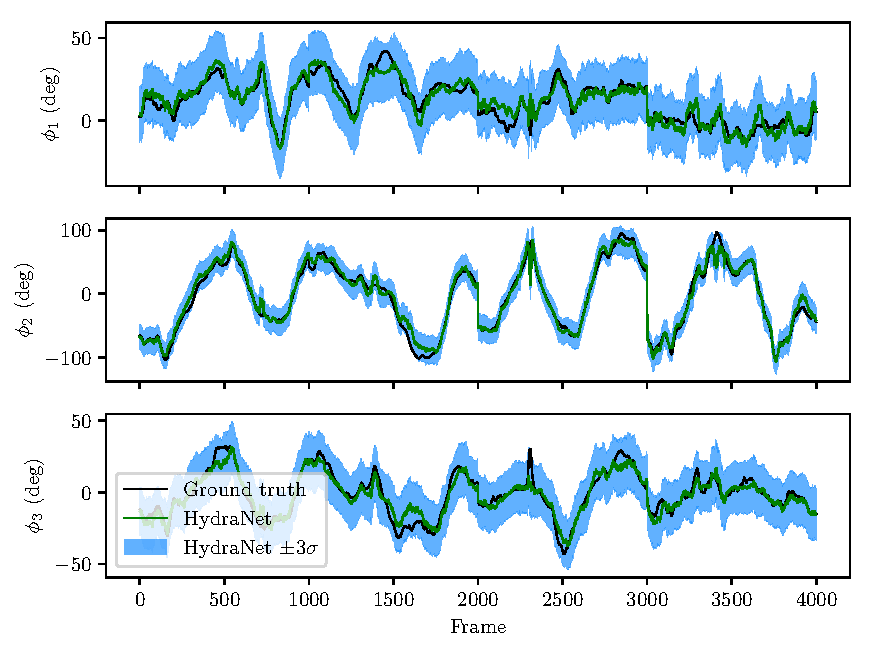
\includegraphics[width=\textwidth]{so3_learning/supplementary/7scenes_abs_best_model_office_heads_25_epoch_15}
		\caption{Office}
	\end{subfigure}
	\begin{subfigure}[]{0.33\textwidth} 
		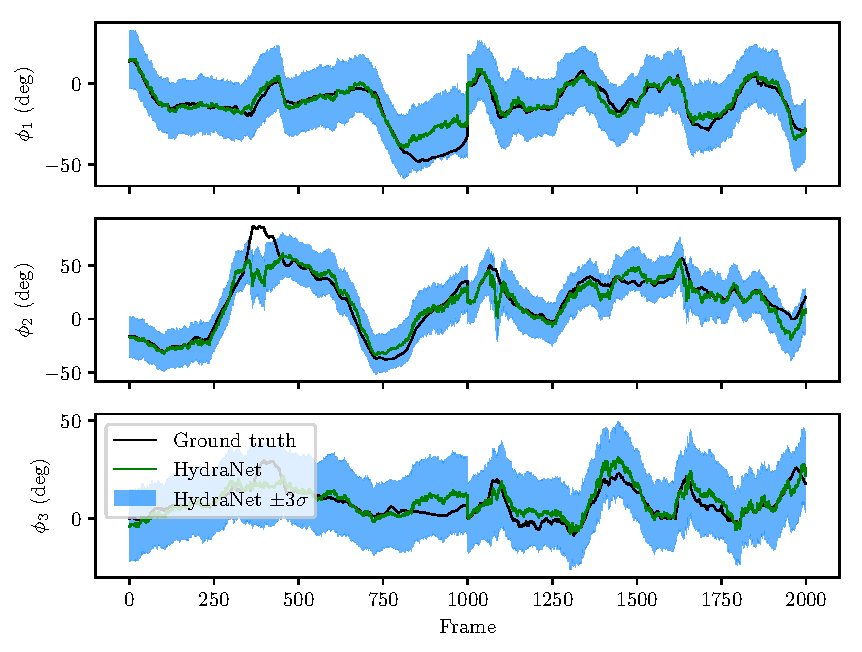
\includegraphics[width=\textwidth]{so3_learning/supplementary/7scenes_abs_best_model_pumpkin_heads_25_epoch_13}
		\caption{Pumpkin}
	\end{subfigure}
	\begin{subfigure}[]{0.33\textwidth} 
		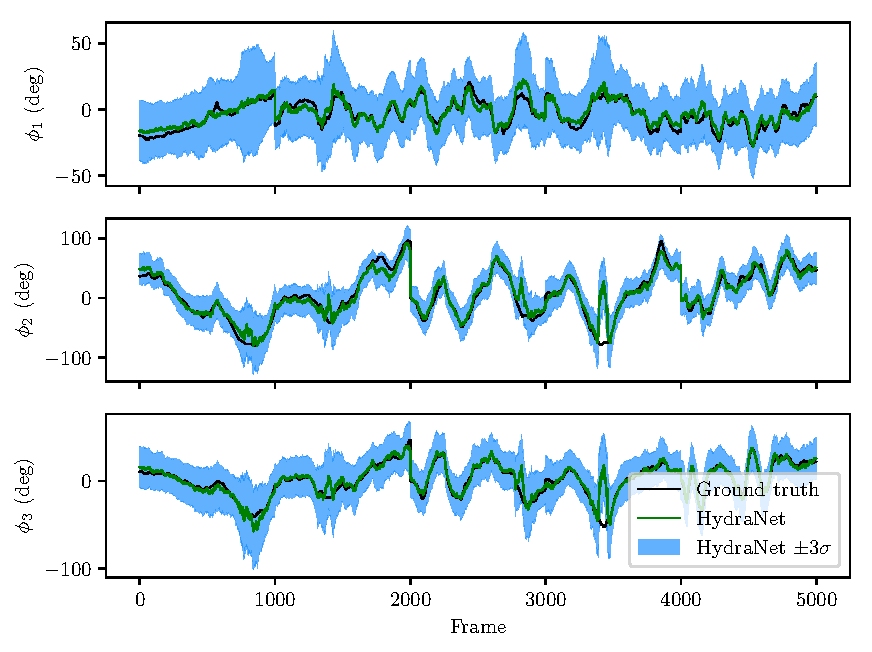
\includegraphics[width=\textwidth]{so3_learning/supplementary/7scenes_abs_best_model_redkitchen_heads_25_epoch_2}
		\caption{Kitchen}
	\end{subfigure}
	\begin{subfigure}[]{0.33\textwidth} 
		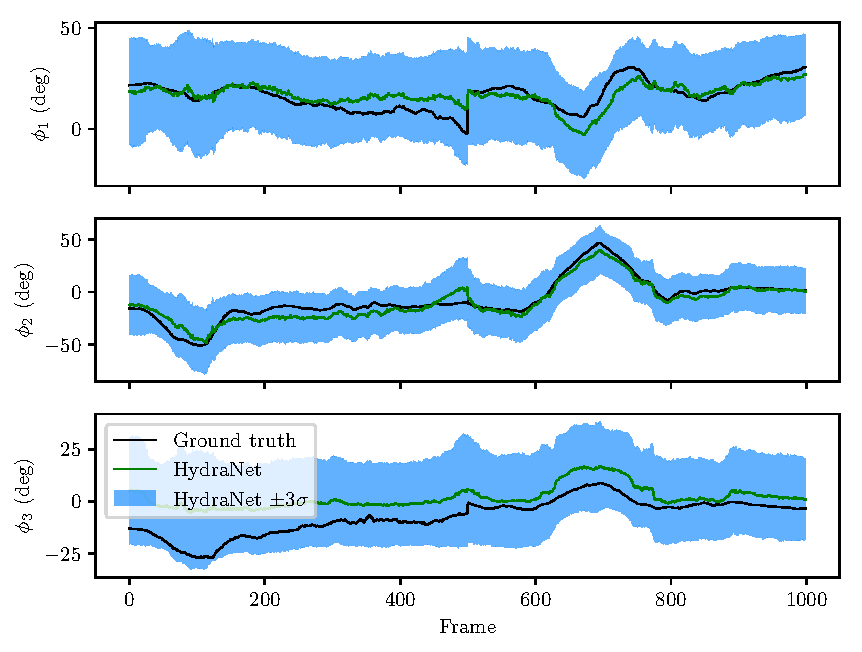
\includegraphics[width=\textwidth]{so3_learning/supplementary/7scenes_abs_best_model_stairs_heads_25_epoch_11}
		\caption{Stairs}
	\end{subfigure}
	
	\caption{Probabilistic regression plots for all seven datasets from the 7-Scenes dataset.}
	\label{fig:7scenes_regression}
\end{figure*}

\subsection{KITTI}
\subsubsection{Network details}
Our custom convolutional network was built using PyTorch as follows:

\begin{python}
self.cnn = torch.nn.Sequential(
    conv_unit(2, 64),
    conv_unit(64, 128),
    conv_unit(128, 256),
    conv_unit(256, 512),
    conv_unit(512, 1024),
    conv_unit(1024, 1024),
    conv_unit(1024, 1024)
)
\end{python}
with each \texttt{conv\_unit} defined as,
\begin{python}
def conv_unit(in, out, ks=3, st=2, pad=1):
        return torch.nn.Sequential(
            torch.nn.Conv2d(in, out, 
            	kernel_size=ks, 
            	stride=st, 
            	padding=pad),
            torch.nn.BatchNorm2d(out),
            torch.nn.ReLU()
        )	
\end{python}
and the head structure being identical to both of the previous experiments. Our two-dimensional flow image was constructed using OpenCV with the function \texttt{calcOpticalFlowFarneback()} from two RGB images converted to grayscale. We trained the network using the Adam optimizer, with a learning rate of $5 \times 10^{-5}$ and no pre-training. We found that augmenting the dataset with rotation targets and inputs that represented both the forward and reverse temporal pairs improved generalization. 
%
%
%\begin{python}
%class GenericHead(torch.nn.Module):
%    def __init__(self, D_in, D_out, 
%    			D_mid, dropout=False):
%        super(GenericHead, self).__init__()
%        self.fc0 = torch.nn.Linear(D_in, D_mid)
%        self.fc1 = torch.nn.Linear(D_mid, D_out)
%        if dropout:
%            self.dropout = torch.nn.Dropout()
%        else:
%            self.dropout = False
%        self.nonlin = torch.nn.PReLU()
%
%    def forward(self, x):
%        out = self.fc0(x)
%        out = self.nonlin(out)
%        if self.dropout:
%            out = self.dropout(out)
%        out = self.fc1(out)
%        return out	
%\end{python}


\begin{figure*}[h!]
	\centering
	\begin{subfigure}[]{0.33\textwidth}
		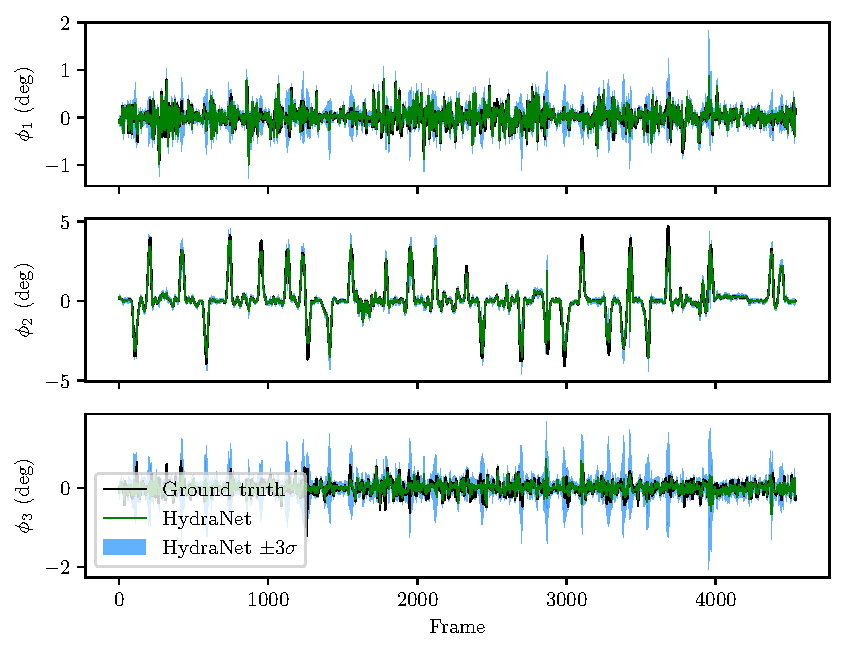
\includegraphics[width=\textwidth]{so3_learning/supplementary/kitti_abs_00_downsample_5}
		\caption{\texttt{00}}
	\end{subfigure}
	\begin{subfigure}[]{0.33\textwidth} 
		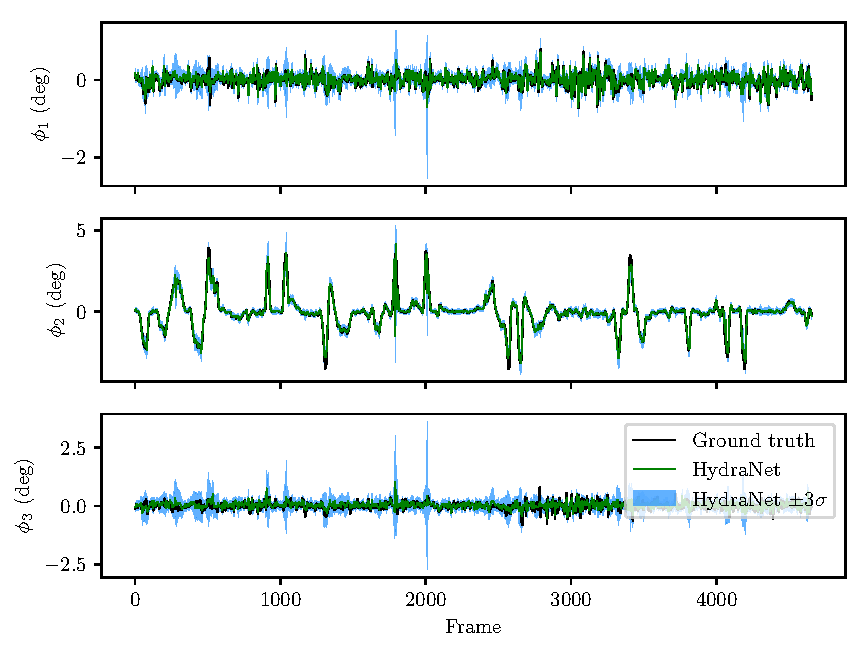
\includegraphics[width=\textwidth]{so3_learning/supplementary/kitti_abs_02_downsample_5}
		\caption{\texttt{02}}
	\end{subfigure}
	\begin{subfigure}[]{0.33\textwidth} 
		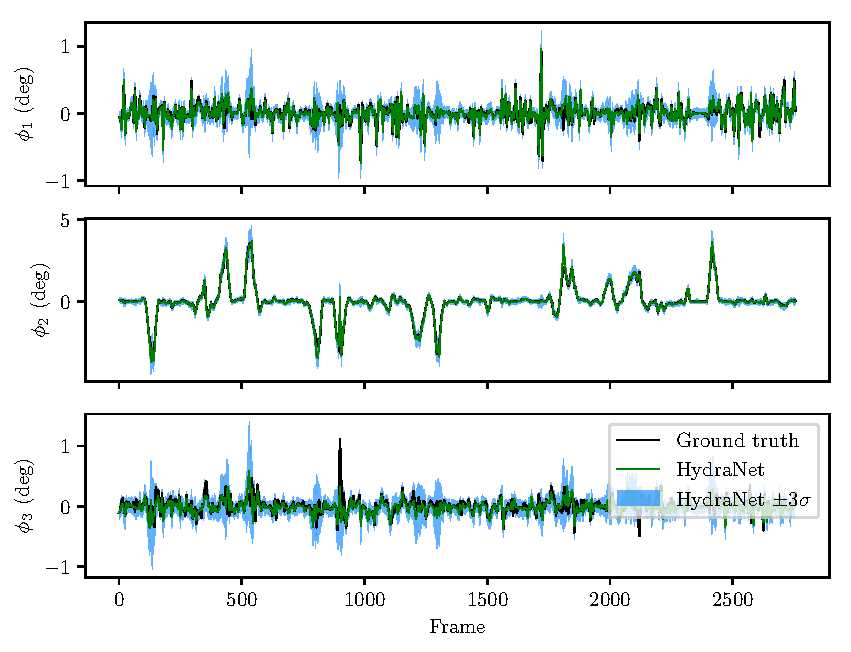
\includegraphics[width=\textwidth]{so3_learning/supplementary/kitti_abs_05_downsample_5}
		\caption{\texttt{05}}
	\end{subfigure}
	\begin{subfigure}[]{0.33\textwidth} 
		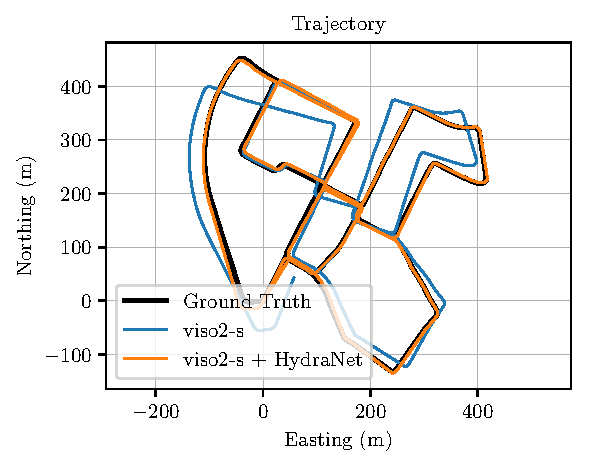
\includegraphics[width=\textwidth]{so3_learning/supplementary/kitti_00_topdown}
		\caption{\texttt{00}}
	\end{subfigure}
	\begin{subfigure}[]{0.33\textwidth} 
		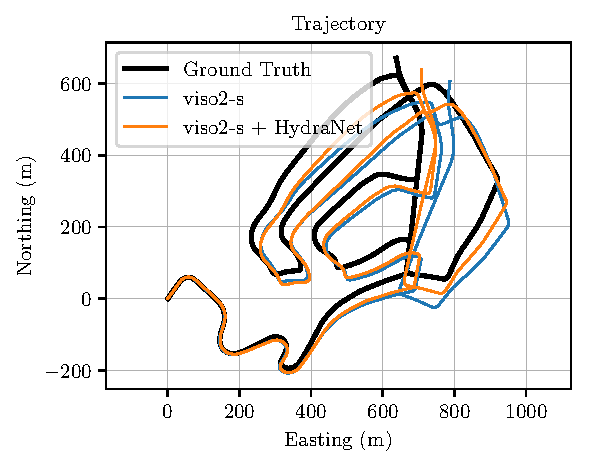
\includegraphics[width=\textwidth]{so3_learning/supplementary/kitti_02_topdown}
		\caption{\texttt{02}}
	\end{subfigure}
	\begin{subfigure}[]{0.33\textwidth} 
		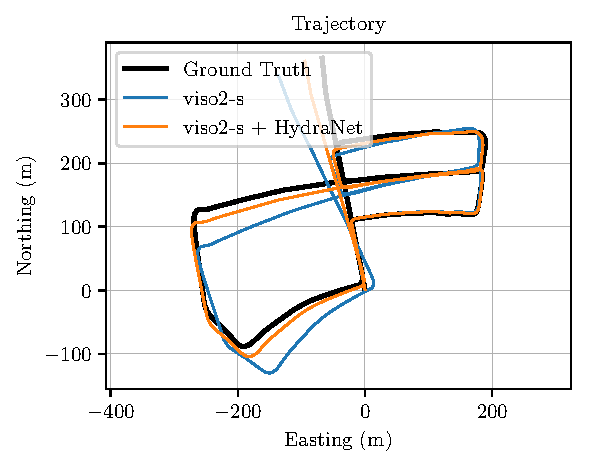
\includegraphics[width=\textwidth]{so3_learning/supplementary/kitti_05_topdown}
		\caption{\texttt{05}}
	\end{subfigure}
	\caption{KITTI frame-to-frame rotation probabilistic regression for sequences \texttt{00}, \texttt{02} and \texttt{05}. Top-down trajectory plots show localization improvements after fusion with a classical stereo visual odometry pipeline.}
	\label{fig:kitti_regression}
\end{figure*}


%\subsubsection{Sparse Visual Odometry}
%
%For the classical visual odometry estimator, we used the open-source \texttt{libviso2} package~\cite{Geiger2011-xe} to detect and track sparse stereo image key-points in a similar manner to \cite{Peretroukhin2018}. We modeled stereo reprojection errors (due to sensor noise
%and quantization) as zero-mean Gaussians with a known covariance, $\ImageCovariance$,
%\begin{align}
% \Vector{e}_{l,t_i} &= \ImageLandmark{l}{t_{i+1}} - \ProjectionFunction( \Transform_{t_{i+1},t_i} 
%    \ProjectionFunction^{-1}( \ImageLandmark{l}{t_{i}} ) ) \\ &\sim \NormalDistribution{\Vector{0}}{\ImageCovariance},
%   \label{eq:image_error}
%\end{align}
%where $\ProjectionFunction(\cdot)$ is the stereo camera projection function. To generate an initial guess and to reject outliers, we used three point Random Sample Consensus (RANSAC) based on stereo reprojection error.
%Finally, we solved for the maximum likelihood transform, $\Transform_{t+1,t}^*$, through a Gauss-Newton minimization of
%\begin{equation}
%  \Transform_{t_{i+1},t_i}^* = \ArgMin{\Transform_{t_{i+1},t_i}\in\text{SE}(3)}\sum_{l=1}^{N_{t_i}} 
%  \Transpose{\Vector{e}}_{l,t_i} \ImageCovariance^{-1} \Vector{e}_{l,t_i}.
%\end{equation}
%
%\noindent Namely, given small pose vector perturbations, $\delta \Vector{\xi}$, about a given operating point, $\Mean{ \Transform}_{t_{i+1},t_i}$, we apply the linear perturbation $ \Transform_{t_{i+1},t_i} \leftarrow (\Matrix{1} + \delta \Vector{\xi}^\wedge) \Mean{\Transform}_{t_{i+1},t_i}$ and solve the linear system,
%\begin{align}
%   \left( \sum_{i=1}^{N_t} \Transpose{\Matrix{J}}_{i,t} \ImageCovariance^{-1} \Matrix{J}_{i,t} \right) \delta \Vector{\xi}^{(n)} = 
%  \sum_{i=1}^{N_t} \Transpose{\Matrix{J}}_{i,t} \ImageCovariance^{-1} \Vector{e}_{i,t}^{(n)}. 
%  \label{eq:least-squares-iteration}
%\end{align}
%
%
%\noindent We repeat this to convergence, and then approximate the state covariance as \cite{Barfoot2017-ri}:
%\begin{equation}
%	\Matrix{\Sigma}_\text{vo} \approx  \left( \sum_{i=1}^{N_t} \Transpose{\Matrix{J}}_{i,t} \ImageCovariance^{-1} \Matrix{J}_{i,t} \right)^{-1}
%    \label{eq:svo_uncertainty}
%\end{equation}
\vspace{-1em}
\subsubsection{Keyframe direct VO}
To compare with an accurate classical method, we used a state-of-the-art dense direct stereo visual odometry method based off of keyframes and minimization of pixel re-projection error. This method is similar to the dense method presented in \cite{2018_Peretroukhin_Deep} and largely based on the ideas in \cite{engel2014lsd}. We plan to release this pipeline after the double-blind review process.

\subsubsection{Pose graph relaxation}

As discussed in the main paper, we fused our probabilistic rotation regression with classical stereo visual odometry using pose graph relaxation implemented with the help of a Python-based factor graph library which we will publicize after the review process. Using that framework, we solved
\begin{align}
	\Transform_{1,w}^*, \Transform_{2,w}^* &= \ArgMin{\Transform_{1,w}, \Transform_{2,w}\in\text{SE}(3)}\mathcal{L}(\Estimate{\Transform}_{2,1}, \Estimate{\Rotation}_{2,1}) \\ & = \ArgMin{\Transform_{1,w}, \Transform_{2,w}\in\text{SE}(3)} \Vector{\xi}_\text{1,2}^T \Matrix{\Sigma}^{-1}_\text{vo} \Vector{\xi}_\text{1,2} + \Vector{\phi}_\text{1,2}^T \Matrix{\Sigma}^{-1}_{\text{hn}} \Vector{\phi}_\text{1,2} 
\end{align}
where
\begin{equation}
	\Vector{\xi}_\text{1,2} =  \MatLog{\left(\Transform_{2,w} \Transform_{1,w}^{-1} \right)\Estimate{\Transform}_{2,1}^{-1}},
\end{equation}
\begin{equation}
	\Vector{\phi}_\text{1,2} =  \MatLog{\left(\Rotation_{2,w} \Rotation_{1,w}^{T} \right)\Estimate{\Rotation}_{2,1}^{T}},
\end{equation}
and $\Estimate{\Transform}_{2,1}$, $\Matrix{\Sigma}_\text{vo}$ and $\Estimate{\Rotation}_{2,1}$, $\Matrix{\Sigma}_{\text{hn}}$ were provided by our classical estimator and the HydraNet network respectively. Note that $\Matrix{\Sigma}_{\text{hn}} \in \Real^{3 \times 3} \geq 0$ while $\Matrix{\Sigma}_{\text{vo}} \in \Real^{6 \times 6} \geq 0 $. We also overload the logarithm function, $\MatLog{\cdot}$ to represent both $\LieGroupSE{3}$ and $\LieGroupSO{3}$ logarithmic maps as necessary. To account for gauge freedom, we fixed the first transformation to identity, $\Transform_{1,w} = \IdentityMatrix$, and initialized $\Transform_{2,w}$ to  $\Estimate{\Transform}_{2,1}$.  After convergence, we composed the final frame-to-frame estimate as $ \Transform_{2,1}^* =  \Transform_{2,w}^*  \left(\Transform_{1,w}^*\right)^{-1} = \Transform_{2,w}^*$.

\subsubsection{Additional results}
We present  additional regression and fused trajectory results for KITTI odometry benchmark sequences \texttt{00}, \texttt{02} and \texttt{05} in \Cref{fig:kitti_regression}. We trained each test sequence with the remainder of the sequences in the dataset, mimicking a cross-validation approach.